\documentclass{article}
\usepackage{amsmath}
\usepackage{amssymb}
\usepackage{enumitem}
\usepackage{graphicx}
\usepackage{xcolor}
\usepackage{adjustbox}
\usepackage{tikz}
% \usepackage{lscape} % for landscape orientation

% Set page dimensions for landscape mode
% \usepackage[paper=landscape, margin=1in]{geometry}

% Set up the theorem environment
\usepackage{amsthm}
\newtheorem{theorem}{Theorem}

% Custom commands for vectors and matrices
\newcommand{\vect}[1]{\mathbf{#1}}
\newcommand{\mat}[1]{\mathbf{#1}}

\title{Linear Algebra - Project}
\author{Meet Gera \and Yashas \and Rohan}
\date{Course Instructor: Dr. Chittraranjan Hens \\  IIIT Hyderabad}

\begin{document}

\maketitle

\begin{abstract}
Eigenvalues offer a window into the intrinsic properties of graphs, providing a means to comprehend their connectivity, partitioning, symmetry, and dynamics. The exploration of the spectral realm has paved the way for advancements in diverse fields, ranging from computer science and mathematics to social sciences and biology. By leveraging the power of eigenvalues, researchers can unravel the hidden intricacies of graphs and harness their insights to tackle real-world challenges.
\end{abstract}

\section{Introduction}
Eigenvalues serve as a key tool in understanding graph connectivity and community structure. By examining the eigenvalues of a graph's adjacency matrix, which captures essential structural information about the graph's connectedness, we can gain valuable insights. The number of zero eigenvalues, known as the algebraic connectivity, provides a measure of the robustness and resilience of the graph. Moreover, the eigenvectors corresponding to the smallest nonzero eigenvalue aid in graph partitioning. Beyond that, eigenvalues unlock further insights into the behavior of graphs. The spectrum of eigenvalues reveals information about the graph's symmetry, regularity, and expansion properties. Large eigenvalues indicate the presence of well-connected clusters or highly influential nodes, while small eigenvalues suggest sparseness or potential bottlenecks. Furthermore, the distribution of eigenvalues allows for the identification of graph families and the comparison of graph similarity. Eigenvalues offer a window into the intrinsic properties of graphs, providing a means to comprehend their connectivity, partitioning, symmetry, and dynamics. The exploration of the spectral realm has paved the way for advancements in diverse fields, ranging from computer science and mathematics to social sciences and biology. By leveraging the power of eigenvalues, researchers can unravel the hidden intricacies of graphs and harness their insights to tackle real-world challenges.

\section{Bipartite Graphs}
\subsection{Mathematical Representation}
A graph is a collection of nodes and edges, denoted as $G=(V,E)$. In the case of bipartite graphs, there are two sets of nodes such that there are no edges between any two nodes of the same set. Mathematically, we can represent this as $\exists V_1, V_2$ such that $V_1 \cup V_2 = V$ and $V_1 \cap V_2 = \emptyset$. The representation of bipartite graphs is given by $G = (V_1, V_2, E)$.

\begin{figure}[h]
\centering
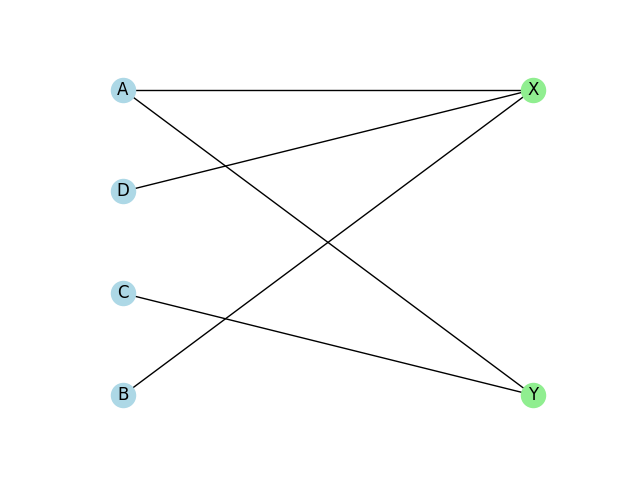
\includegraphics[width=0.6\textwidth]{Graph.png}
\caption{Example of a Bipartite Graph}
\label{fig:bipartite_graph}
\end{figure}

\subsection{Adjacency Matrix}
The adjacency matrix $\mat{A}$ is a square matrix of size $n \times n$, where $n$ is the number of nodes in the graph. For a bipartite graph, the adjacency matrix is partitioned into four blocks, capturing the connections between nodes in $V_1$, nodes in $V_2$, and edges between $V_1$ and $V_2$. The adjacency matrix of a bipartite graph takes the form:

\[
\mat{A} = 
\begin{bmatrix}
\mat{0} & \mat{B} \\
\mat{B}^T & \mat{0}
\end{bmatrix}
\]

where $\mat{0}$ represents the zero matrix and $\mat{B}$ captures the edges connecting $V_1$ and $V_2$. The adjacency matrix provides a concise representation of the graph's structure and facilitates various graph analysis techniques.

\subsection{Eigenvalues of Bipartite Graphs}
The eigenvalues of a bipartite graph's adjacency matrix exhibit an interesting property. Let $\mat{A}$ be the adjacency matrix of a bipartite graph. By definition, a bipartite graph has its vertices divided into two disjoint sets such that all edges connect vertices from different sets. The eigenvalues of $\mat{A}$ appear in pairs of $+a$ and $-a$, where $a$ is a real number. This property holds true due to the specific structure of bipartite graphs and has important implications for understanding their spectral properties.

\begin{figure}[h]
    \centering
    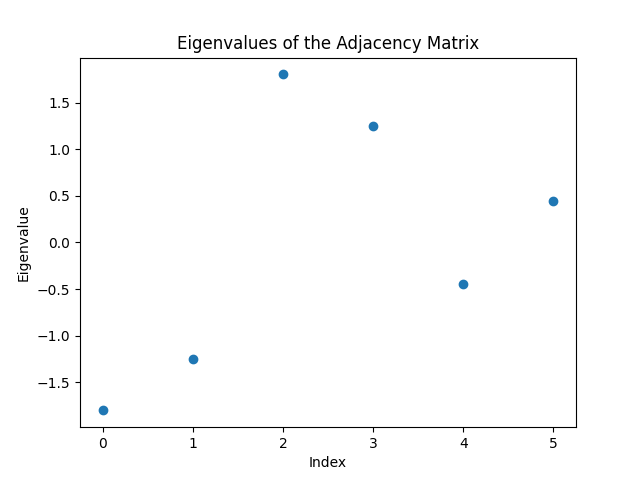
\includegraphics[width=0.6\textwidth]{Eigenvalues.png}
    \caption{Example of a eigenvalues in Complex Plane}
    \label{fig:Eigenvalues}
    \end{figure}
    

\section{Relation with Eigenvalue and Proof}
\begin{theorem}[Eigenvalues of Bipartite Graphs]
Let $\mat{A}$ be the adjacency matrix of a bipartite graph. By definition, a bipartite graph has its vertices divided into two disjoint sets such that all edges connect vertices from different sets. The eigenvalues of $\mat{A}$ appear in pairs of $+a$ and $-a$, where $a$ is a real number.
\end{theorem}

\begin{proof}
We will prove the statement by considering the properties of the adjacency matrix of a bipartite graph.

\begin{enumerate}[label=\textbf{Step \arabic*:}, wide=0pt, leftmargin=!, itemindent=2em]
    \item \textbf{Matrix $A^2$}
    
    Consider the matrix $\mat{A}^2$. The $(i, j)$th entry of $\mat{A}^2$ represents the number of paths of length 2 between vertex $i$ and vertex $j$. In a bipartite graph, there are no direct edges between vertices within the same set, so all entries on the diagonal of $\mat{A}^2$ are zero.
    
    \item \textbf{Equivalence of $A^2v$ and $Av^2$}
    
    For any vector $\vect{v}$, we have $(\mat{A}^2)\vect{v} = \mat{A}(\vect{v}^2)$. This equation can be proven using matrix multiplication.
    
    \item \textbf{Eigenvalue $\lambda$ and eigenvector $\vect{v}$}
    
    Let $\lambda$ be an eigenvalue of $\mat{A}$ with eigenvector $\vect{v}$. By definition, $\mat{A}\vect{v} = \lambda\vect{v}$.
    
    \item \textbf{From $Av = \lambda v$ to $Av^2 = \lambda(Av)$}
    
    Multiply both sides of the equation by $\mat{A}$: $\mat{A}(\mat{A}\vect{v}) = \mat{A}(\lambda\vect{v})$. This yields $\mat{A}^2\vect{v} = \lambda(\mat{A}\vect{v})$.
    
    \item \textbf{Substituting Step 2}
    
    By substituting Step 2, we have $\mat{A}\vect{v}^2 = \lambda(\mat{A}\vect{v})$. This implies that $\lambda$ is an eigenvalue of $\mat{A}^2$ with eigenvector $\vect{v}^2$.
    
    \item \textbf{Non-negativity of $A^2$}
    
    The eigenvalues of $\mat{A}^2$ are non-negative. This is because $\mat{A}^2$ is a non-negative matrix representing the number of paths of length 2 in the bipartite graph.
    
    \item \textbf{Eigenvalue $\lambda$ is non-negative}
    
    Since $\lambda$ is an eigenvalue of $\mat{A}^2$, we have $\lambda \geq 0$.
    
    \item \textbf{Assumption: $\lambda \neq 0$}
    
    Let's assume $\lambda \neq 0$. If $\lambda \neq 0$, then the eigenvector $\vect{v}^2$ is nonzero.
    
    \item \textbf{From $Av = \lambda v$ to $\lambda = \frac{v^TA^Tv}{v^Tv}$}
    
    By the definition of the eigenvalue, we have $\mat{A}\vect{v} = \lambda\vect{v}$. Multiplying both sides of the equation by $\vect{v}^T$, we get $(\vect{v}^T\mat{A}\vect{v}) = \lambda(\vect{v}^T\vect{v})$.
    
    \item \textbf{Symmetric property}
    
    Since $\mat{A}^T = \mat{A}$ for a bipartite graph, we have $\mat{A}^T\vect{v} = \mat{A}\vect{v}$. This implies that $(\vect{v}^T\mat{A}^T\vect{v}) = (\vect{v}^T\mat{A}\vect{v})$.
    
    \item \textbf{Combining Step 9 and Step 10}
    
    Combining steps 9 and 10, we get $\lambda = \frac{v^TA^Tv}{v^Tv}$.
    
    \item \textbf{Eigenvalue $\lambda$ is real}
    
    Since $\lambda = \frac{v^TA^Tv}{v^Tv}$, it follows that $\lambda$ is a real number.
    
    \item \textbf{Conclusion: Eigenvalues appear in pairs}
    
    Therefore, we conclude that the eigenvalues of $\mat{A}$ appear in pairs of $+a$ and $-a$, where $a$ is a real number.
\end{enumerate}

\end{proof}

\begin{figure}[htbp]
  \centering
  \begin{tikzpicture}[scale=1.5]
    % Draw axes
    \draw[->] (-4, 0) -- (4, 0) node[right] {$\text{Re}$};
    \draw[->] (0, -1.5) -- (0, 1.5) node[above] {$\text{Im}$};
    
    % Draw eigenvalues
    \filldraw[color=red] (-2, 0) circle (1pt) node[above] {$-a$};
    \filldraw[color=red] (2, 0) circle (1pt) node[above] {$a$};
    
    % Draw axes labels
    \foreach \x in {-3, -2, ..., 3}
      \draw (\x, 0.1) -- (\x, -0.1) node[below] {$\x$};
    \foreach \y in {-1, 1}
      \draw (0.1, \y) -- (-0.1, \y) node[left] {$\y i$};
  \end{tikzpicture}
  \caption{Eigenvalues of a Bipartite Graph}
  \label{fig:eigenvalues}
\end{figure}
\section{Conclusion for Bipartite Graphs}
In conclusion, the study of bipartite graphs and their eigenvalues holds great promise for understanding graph connectivity, community structure, and various real-world applications. The exploration of eigenvalues provides valuable insights into the robustness, resilience, and behavior of bipartite graphs.

The application of bipartite graphs extends to various domains, including matching and assignment problems, biological networks, and social network analysis. By leveraging the power of eigenvalues, researchers can unravel the hidden intricacies of bipartite graphs and harness their insights to tackle real-world challenges.

Looking to the future, the utilization of bipartite graphs and their eigenvalues is expected to continue advancing. As data becomes increasingly complex and interconnected, bipartite graphs offer a powerful framework for modeling and analyzing large-scale networks. From personalized recommendations to understanding information diffusion, bipartite graphs have the potential to revolutionize various fields and drive innovative solutions.

In conclusion, the study of bipartite graphs and their eigenvalues opens up new avenues for research and practical applications. By delving into the spectral realm of eigenvalues, we can unlock the hidden patterns and structures within bipartite graphs, paving the way for further advancements in graph theory and its applications.

So, let us embrace the power of eigenvalues and embark on a journey to unravel the mysteries of bipartite graphs. With each step, we deepen our understanding of their connectivity, partitioning, symmetry, and dynamics, ultimately enabling us to tackle real-world challenges with confidence and precision.
\end{document}